%!TEX root = thesis.tex

\chapter{Results for FGK stars}
\label{cha:results}
\epigraph{Promises are only words until more than words are required.}{Terry Brooks}

It is time to apply the theory and methodology on some real data. There is the compilation of a NIR
iron line list for deriving stellar atmospheric parameters. This line list was tested against the
well-studied solar-type star, HD 20010 in \citet{Andreasen2016}. Later a second version of the line
list was made. This was tested again on HD 20010 and additionally on two colder stars, Arcturus and
10 Leo in \citet{Andreasen2017b}. A small summary of the stars and their characteristics can be
found in \tref{tab:stars}. More details are provided in the individual sections below for each star.
An update to SWEET-Cat \citep{Santos2013}, a catalogue which provides homogeneous stellar parameters
of planet hosts, was provided in \citet{Andreasen2017a}. \st{Additionally in this work, there was an
analysis of how a selection of lines with different excitation potential might affect the final
parameters of a star, which is discussed in -} Last is the analysis of a range of
synthetic spectra from the PHOENIX spectral library \citep{Husser2013}, with $T_\mathrm{eff}$ lower
than analysed in previous stars with the methodology described above in \sref{sec:parameters}.
However, before diving into the results of the analysis it is important to describe how the NIR line
list was compiled, and why and how it was later refined.

\begin{table*}[htb!]
    \caption{Summary of the four stars used in this thesis. The stellar parameters are an average
             from the PASTEL catalogue \citep{Soubiran2016} (see text for details), except the
             parameters for the Sun.}
    \label{tab:stars}
    \centering
    \begin{tabular}{lllllll}
      \hline\hline
        Star        & Spectrographs  & Resolution  & $T_\mathrm{eff}$ (K) &  $\log g$ (dex)  &   $\xi_\mathrm{micro}$ (km/s)   & [Fe/H] (dex)      \\
      \hline
        Sun         & FTS            & 600\,000    & $5777$               &  $4.44$          &    $1.00$                       & $ 0.00$          \\
        Arcturus    & FTS            & 100\,000    & $4300 \pm 111$       &  $1.60 \pm 0.29$ &    $1.93 \pm 0.17$              & $-0.54 \pm 0.11$ \\
        HD 20010    & CRIRES         & 100\,000    & $6152 \pm  95$       &  $3.96 \pm 0.11$ &    $1.17 \pm 0.24$              & $-0.27 \pm 0.06$ \\
        10 Leo      & CRIRES         & 100\,000    & $4742 \pm  61$       &  $2.76 \pm 0.17$ &    $1.45 \pm 0.08$              & $-0.03 \pm 0.02$ \\
      \hline
    \end{tabular}
\end{table*}

\section{The creation of a NIR line list}
\label{sec:linelist_first}

Although previous work \citep[see e.g.][]{Onehag2012,Lindgren2016,Shetrone2015} have compiled some
NIR line lists for different purposes, there still does not exists an iron line list to determine
stellar atmospheric parameters from high S/N and high resolution spectra. With the advancement of
NIR high resolution spectrographs the time has arrived to compile such a line list, which should be
properly tested (used to determine parameters of well known stars).

As discussed extensively in \cref{cha:theory} and \cref{cha:method}, an atomic line list is needed
for employing the method of deriving the stellar atmospheric parameters used in this thesis. This
line list is composed by neutral and ionized iron lines in the NIR. This has already been mentioned
in \cref{cha:theory}. Here the process will be explained in greater detail below for the two
versions presented in \citet{Andreasen2016} and \citet{Andreasen2017b}, respectively.


\subsection{Measuring the EWs and first filtering}

The first version of a NIR iron line list for determining stellar atmospheric parameters of high
resolution and high S/N spectra were presented in \citet{Andreasen2016}. Other NIR line lists exists
such as the one from \citet{Onehag2012,Lindgren2016} for utilising the synthetic method described
above of high resolution spectra. Their line list cover the J band in the NIR and consists of 48
lines of different elements. For this line list all iron transitions between
\SIrange{10000}{25000}{\angstrom}\footnote{That is equivalent to the YJHK bands.} were downloaded
from the VALD database \citep{VALD1,VALD2}, only including \ion{Fe}{I} and \ion{Fe}{II} transitions.
In total were \num{50198} \ion{Fe}{I} and \num{28339} \ion{Fe}{II} lines respectively acquired.

The EW of all lines were measured in the solar atlas by \citet{Hinkle1995}. The EWs were measured
using \code{ARES} due to the large amount of lines and to be as consistent as possible in the
measurements. Since \code{ARES} expect a 1D spectrum with equidistant wavelength step, the solar
spectrum was interpolated onto a regular wavelength grid of \SI{0.01}{\angstrom}. This did not
change the appearance, and hence not the EW, of the final spectrum. This wavelength step is
equivalent to a spectral resolution of \num{1500000} at \SI{15000}{\angstrom}. The S/N for the solar
atlas varies between 300 to 2000 across the spectrum, but is generally of a very high quality.

The EWs were measured by fitting Gaussian profiles to the spectral lines. For a given line,
\code{ARES} output the central wavelength of the line (provided in the line list), the FWHM maximum
of the fitted line, the number of lines fitted for the final result (in case of blending), the depth
of the line, and the EW of the line of the line. In the latest version of \code{ARES}, the error of
the EW is also provided \citep{Sousa2015a}.

As a first selection step, lines were discarded according to the following four criteria:

\begin{itemize}
  \item Lines with EW lower than \SI{5}{m\angstrom}: these lines can be problematic to see in
        spectra with lower S/N or spectra with many spectral features. Therefore the measurements
        of these lines are less reliable than stronger lines.
  \item Lines with EW higher than \SI{200}{m\angstrom}: These lines are too strong to be fitted
        with a Gaussian profile. These lines might also be saturated and do not fall in the linear
        regime of the curve-of-growth (see \fref{fig:cog}).
  \item Lines where the total number of fitted lines are 10 or higher meaning the presence of
        severe blending.
  \item If the fitted central wavelength is more than \SI{0.05}{\angstrom} away from the wavelength
        provided by VALD3 to avoid false identification. This should also remove some blended lines.
  \item Removal of lines with EP higher than \SI{5.5}{eV}. This cut was inspired by available EPs in
        the optical \citep[see e.g.][]{Sousa2008a}.
\end{itemize}
After this removal the number of \ion{Fe}{I} and \ion{Fe}{II} lines were reduced to \num{6060} and
\num{2735}, respectively.


\subsection{Visual removal of lines}
\label{sec:visual}

At this point a visual inspection was necessary. All atomic data for possible transitions from all
elements were downloaded from the VALD3 database in a \SI{3}{\angstrom} window around each of the
nearly \num{9000} iron lines from the previous step. For each small spectral window, all absorption
lines (including the iron line(s)) were located in a plot of the solar spectrum. An iron line was
discarded if another line had the same central wavelength and/or the absorption line were severely
blended. Most of the discarded iron lines had high EP, which are weak compared to the low EP lines.
Therefore, it is fair to assume that many of these iron lines were falsely identified as another
stronger line from another element. After the visual removal the number of \ion{Fe}{I} and
\ion{Fe}{II} lines were reduced to a mere 593 and 22, respectively. In \fref{fig:visualSelection} is
a case where too many lines are present near the iron line of interest (green line in the middle).
The green lines are all iron lines in the spectral region, while the orange lines are other elements
or molecules. The depth and transparency is a measure by the line strength given by
\begin{align}
  \mathrm{strength} = \log\mathrm{gf} - \chi \Theta, \label{eq:strength}
\end{align}
where $\Theta=\SI{5040}{K}/T_\mathrm{eff}$ (solar temperature is used here). Note that this strength
of the lines does not include any abundance information, and should therefore be a guide rather than
an actual measure.

\begin{figure}[htpb!]
    \centering
    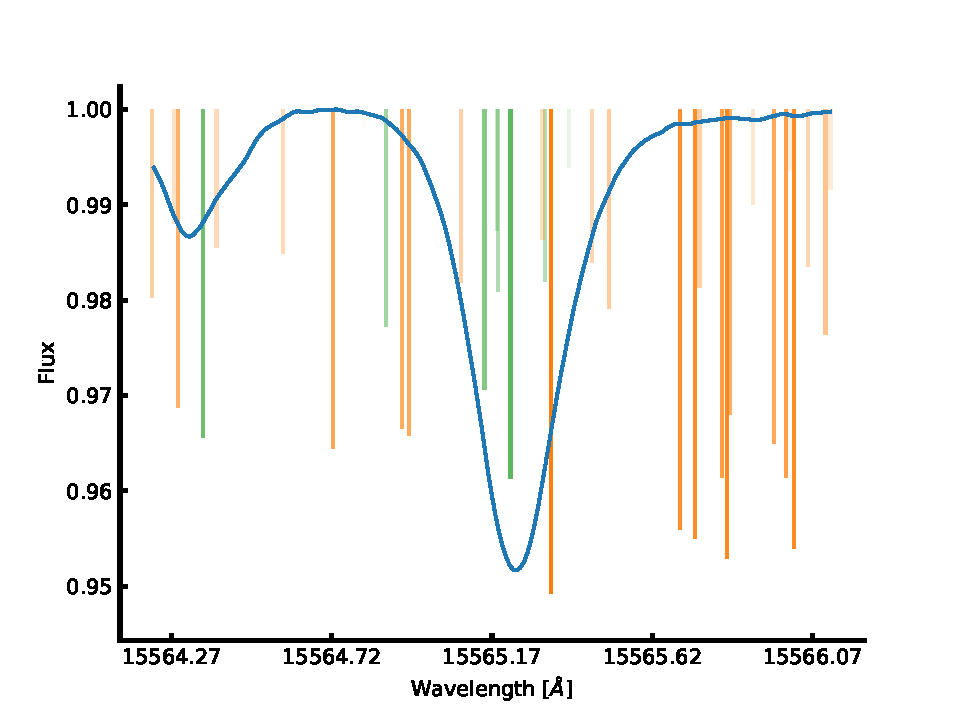
\includegraphics[width=0.8\linewidth]{figures/visualSelection.pdf}
    \caption{Solar spectrum (blue) with all iron lines in the spectral region (green) and other
             elements (orange). The depths and transparencies of the vertical lines are a measure of
             the line strengths (see \eref{eq:strength} for details). This is a case where the iron
             line is discarded due to blending, which is clear in the left wing of the central
             absorption line.}
    \label{fig:visualSelection}
\end{figure}

For some of the absorption lines it was not clear which element was causing it. These lines were
marked for further investigation with synthesis as described below.

\subsection{Synthetic investigation}

For the lines marked above for further investigation an even broader window of \SI{6}{\angstrom} was
used. Once again, all atomic data for possible transitions were downloaded from the VALD3 database
in these spectral windows. \code{MOOG} was used with the \code{synth} driver to create a synthetic
spectrum using a solar atmosphere model with $T_\mathrm{eff}=\SI{5777}{K}$, $\log g=4.438$,
$A(\mathrm{Fe})=7.47$, and $\xi_\mathrm{micro}=\SI{1.00}{km/s}$. The iron abundance (7.47) is from
\citet{Gonzalez2000}, while the overall metallicity for the solar atmosphere model is
$[\ion{M}/\ion{H}]=0.00$ by definition. This step is different from the step visual inspection done
in \sref{sec:visual} since synthetic spectra were created here. This was done for all spectral
windows for three different iron abundances $[\ion{Fe}/\ion{H}]=\{-0.20;\,0.00;\,0.20\}$ in order to
identify iron lines and their impact on the synthetic spectra. Before creating a synthetic spectrum
all elements which are more than singly ionised were removed since \code{MOOG} does not allow these.
An example of the three synthetic spectra can be seen in \fref{fig:synthetic_investigation}. Here
the neutral iron line at \SI{15550.439}{\angstrom} was investigated. The three coloured curves are
synthetic spectra with the three different $[\ion{Fe}/\ion{H}]$. The upper plot shows the result
with the full VALD3 line list, while in the lower plot the iron line was removed from the line list.
The grey curve is the solar atlas for reference. Note that it is not the purpose to match a
synthetic spectrum to the solar atlas.

\begin{figure}[htpb!]
    \centering
    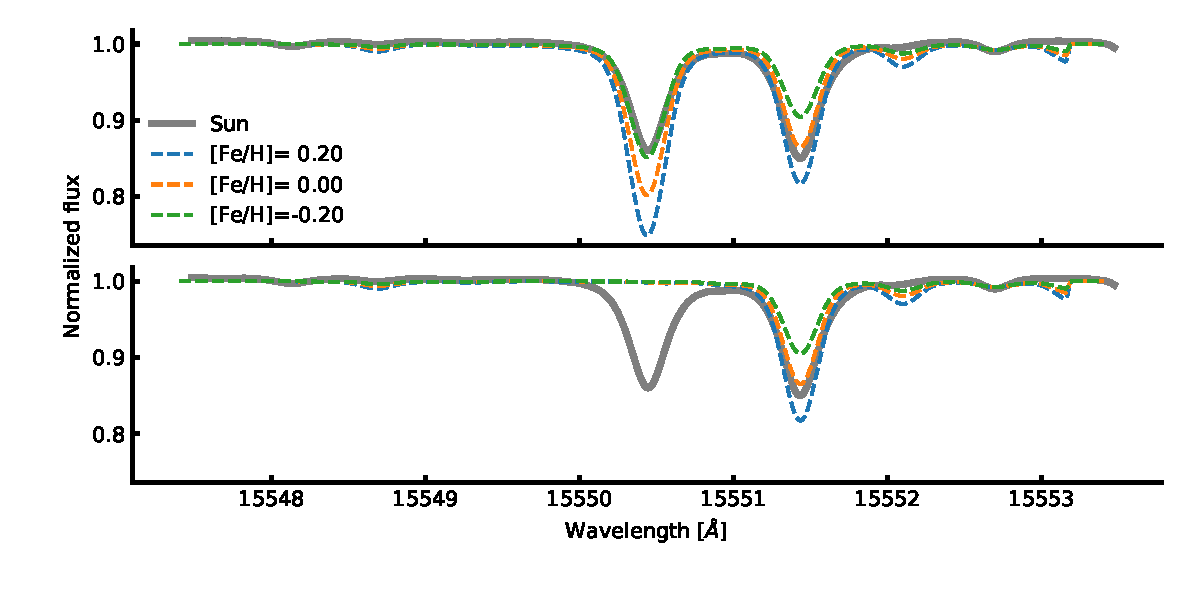
\includegraphics[width=1.0\linewidth]{figures/synthetic_investigation.pdf}
    \caption{The three coloured curves represent different iron abundance, $\{-0.20;\,0.00;\,0.20\}$
             compared to solar abundance. The grey curve is the solar atlas for reference. In this
             case the iron line at \SI{15550.439}{\angstrom} was investigated.
             \emph{Upper panel}:
             Synthetic spectra were computed using the full VALD line list in the spectral range for
             the three different iron abundances.
             \emph{Lower panel}:
             Same as the upper panel, but with the iron line removed from the line list. Since the
             synthetic spectra shows no features at this absorption line anymore, it is a fair
             assumption to say the iron line is the cause of this absorption line.}
    \label{fig:synthetic_investigation}
\end{figure}

If the synthetic spectra shows variation at the iron line of interest, then it is assumed that the
iron line is the cause for the absorption line. As a simple test, the iron line was also removed
from the line list used to create the synthetic spectra. If the iron line in the synthetic spectra
disappeared, it was a clear signal that this line can be used in the final iron line list ( this can
be seen clearly in the lower plot of \fref{fig:synthetic_investigation}). In some cases two iron
lines had the same or very similar wavelength, and this technique was used to include the correct
iron line. In cases where both iron lines causes the absorption line, they were both discarded since
they are blended. In theory both iron lines will contribute to the absorption, however one of the
contributions might be negligible, hence only one of the lines will be discarded.

In a few cases two iron lines had the same wavelength and EP but different $\log \mathit{gf}$. In
these cases the two iron lines they can be combined into a single line by adding their $\mathit{gf}$
values. After this step, there were 414 \ion{Fe}{I} lines and 12 \ion{Fe}{II} lines, respectively.



\subsection{Calibrating the line list: astrophysical \texorpdfstring{$\log \mathit{gf}$}{log gf} values}

These lines were collected into a single line list in the format required by MOOG \citep{Sneden1973}
and the line abundance were measured by all lines using the solar atmosphere model described above.
If the derived abundance for a single line differs by more than \SI{1.0}{dex} from the solar iron
abundance, the line was discarded. All lines before this step can be seen in
\fref{fig:calibrated_loggf} with all lines discarded marked in red.

\begin{figure}[htpb!]
    \centering
    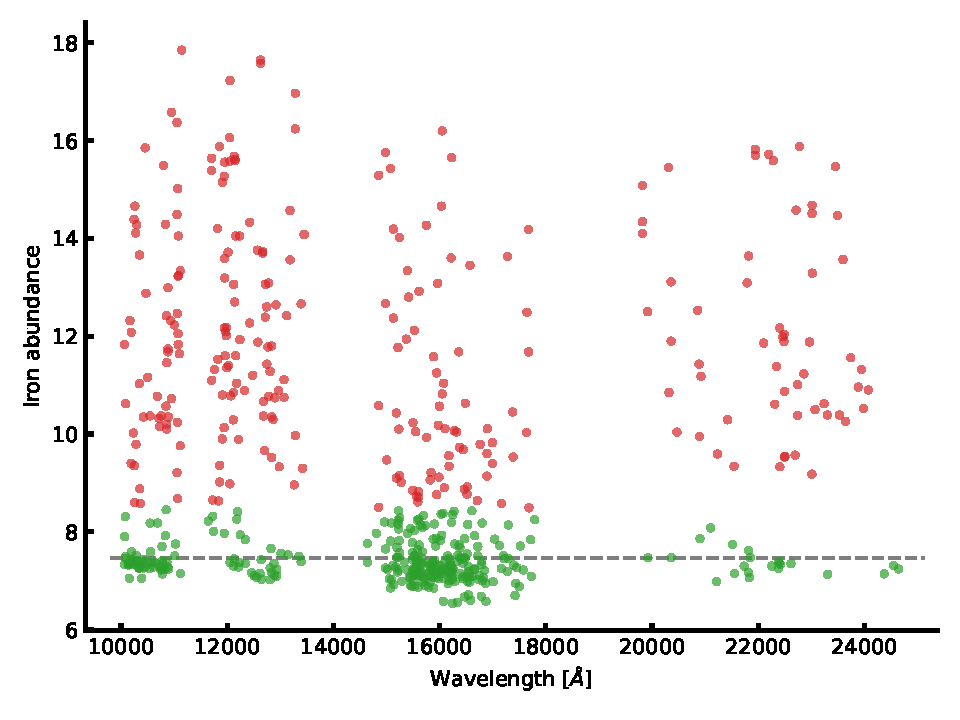
\includegraphics[width=1.0\linewidth]{figures/calibrated_loggf.pdf}
    \caption{Line abundance of all iron lines before calibrating the $\log \mathit{gf}$ values. The
             green points are the points with a deviation less than \SI{1.0}{dex} from the solar
             iron abundance. All the red points are discarded. The horizontal line shows the solar
             iron abundance.}
    \label{fig:calibrated_loggf}
\end{figure}


After the removal of the lines mentioned above, the final line list is almost compiled. At this
point the line list has to be calibrated. This is done by changing $\log \mathit{gf}$ so the line
abundance for all iron lines are 7.47 when using the solar atmosphere model mentioned above. As
mentioned in \sref{sec:linelist} there is a anti-correlation between the abundance of a line and
$\log \mathit{gf}$. This means a simple bisector minimization can be used to locate the
$\log\mathit{gf}$ that gives the desired abundance. This was done for all the iron lines at this
stage.

\paragraph{Note}
If the setup used to determine the parameters is changed, the it is important to calibrate the $\log
\mathit{gf}$ values for the line list again. This includes the type of model atmospheres used (e.g.
ATLAS9 or MARCS), the interpolation code to generate a model atmosphere from the grid, or the
settings of the radiative code, here \code{MOOG}, and even the settings used in the radiative
transfer code, i.e. the specific physics used. In the results listed below the setups are identical,
except for the work done with synthetic spectra (see \sref{sec:synthetic_spectra}). There both
ATLAS9 and MARCS model atmospheres were used, and a calibrated set of $\log \mathit{gf}$ values are
available for both setups.


\subsection{Removal of high dispersion lines}

The line list calibrated above was used to derive parameters for HD 20010 (see \sref{sec:HD20010_first}),
however the derived parameters showed poor results when compared to the literature values. This lead
to the following test:

A Gaussian distribution was made for the EW of each line centred on the EW itself,
\begin{align}
  f(x, EW, \sigma) = \frac{1}{\sqrt{2\pi\sigma^2}} e^{-\frac{(x-EW)^2}{2\sigma^2}},
\end{align}
where $\sigma$ is the error on the EW, expressed by \citet{Caryel1988}:
\begin{align}
  \sigma \simeq 1.6 \frac{\sqrt{\Delta\lambda EW}}{S/N},
\end{align}
where $\Delta\lambda=0.1$ and a S/N=50 were considered here, which is much lower than the actual S/N
of the solar atlas. The search for lines to remove from the line list, in order to improve the
results is as follows:
\begin{enumerate}
  \item Make 100 draws for each EW (giving a total of 100 line lists)
  \item Derive the line abundances for all 100 line lists using the solar model atmosphere and \code{MOOG}
  \item Calculate the mean absolute deviation (MAD) for each line using the derived abundances
  \item Locate the lines with highest dispersion in a MAD versus original EW plot (see
        \fref{fig:dispersive_lines})
\end{enumerate}

\begin{figure}[htpb!]
    \centering
    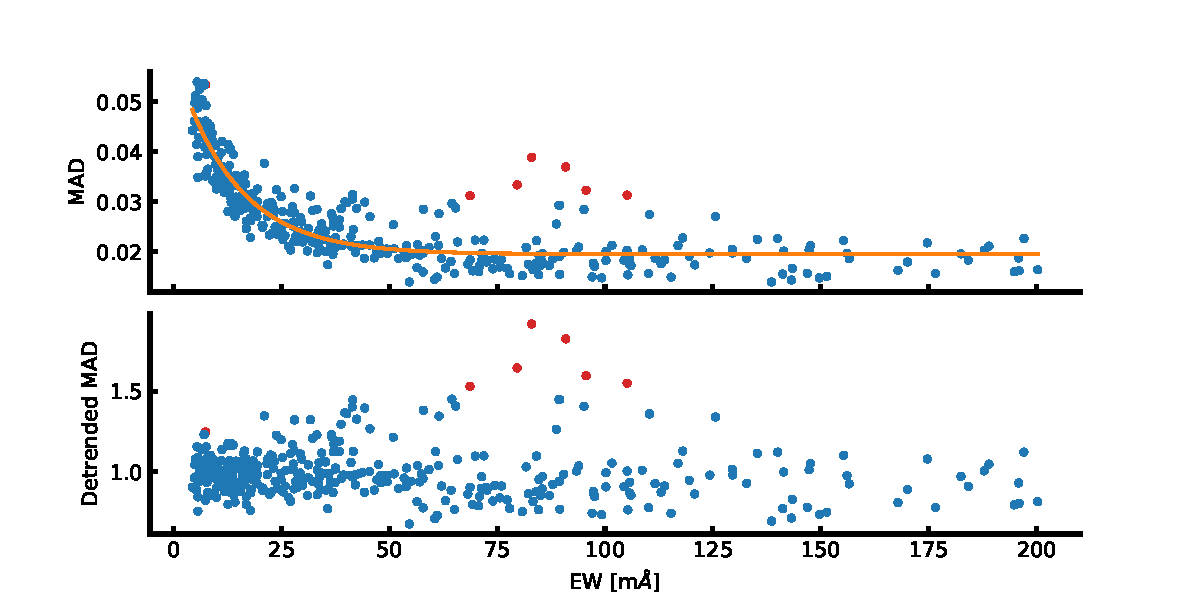
\includegraphics[width=1.0\linewidth]{figures/disperse_lines.pdf}
    \caption{The most disperse lines.
             \emph{Upper panel}:
             The MAD versus the original EW. The red points are the outliers which were discarded
             during this process.
             \emph{Lower plot}:
             Same as above with the de-trended MAD  by the exponential fit as shown in the upper
             panel.}
    \label{fig:dispersive_lines}
\end{figure}

In the upper panel of \fref{fig:dispersive_lines} the weaker lines (i.e. lines with lower EW) shows
a higher MAD value, however this is expected since a small absolute change in the EW results in a
large relative change in abundance for these lines. This does not mean these lines necessarily have
a high dispersion, since it is just the expected outcome of this test. Moreover, these relatively
weak lines from the solar atlas should be stronger for some other spectral types, and therefore
important to include if possible. Therefore the disperse lines are found in the de-trended MAD
value, where an exponential function was used for de-trending. A single point above $3\sigma$ was
removed iteratively in the de-trended data. After this process there are 334 \ion{Fe}{I} lines and
13 \ion{Fe}{II} lines.



\section{HD20010}
\label{sec:HD20010_first}

To test the NIR line list a well-studied solar-type star was needed. The spectrum for such a target
needs to be available in the NIR at both high resolution and high S/N. An ideal place to look for
such a star was the CRIRES-POP database \citep{Lebzelter2012}. Here, the best target for testing was
HD 20010, an F8 subgiant star. At the time of writing this thesis and \citet{Andreasen2016} the
spectrum of HD 20010 was not fully reduced. Here it is still contaminated by some telluric lines,
and the wavelength solution used is not optimal; both which are essential, however a tedious and
difficult task to accomplish.

HD 20010 star has been part of many surveys and is therefore well studied. Different parameters from
the literature are listed in \tref{tab:HD20010}.

\begin{table*}[htb!]
    \caption{Selection of literature values for the atmospheric parameters for HD 20010. The mean
             and a $3 \sigma$ standard deviation is presented at the end of the table from the
             literature values included, which was used as a reference for the derived parameters.}
    \label{tab:HD20010}
    \centering
    \begin{tabular}{l|llll}
      \hline\hline
     Author                 & $T_\mathrm{eff}$ (K) & $\log g$ (dex)  & $[\ion{Fe}/\ion{H}]$ (dex)  & $\xi_\mathrm{micro}$ (km/s)  \\
      \hline
    \cite{Balachandran1990} & $6152$               & $4.15$          & $-0.27 \pm0.08$             & $1.60$                       \\
    \cite{Favata1997}       & $6000$               & \ldots          & $-0.35 \pm0.07$             & \ldots                       \\
    \cite{Santos2004}       & $6275\pm57$          & $4.40\pm0.37$   & $-0.19 \pm0.06$             & $2.41\pm0.41$                \\
    \cite{Gonzalez2010}     & $6170\pm35$          & $3.93\pm0.02$   & $-0.206\pm0.025$            & $1.70\pm0.09$                \\
    \cite{Ramirez2012}      & $6073\pm78$          & $3.91\pm0.03$   & $-0.30 \pm0.05$             & \ldots                       \\
    \cite{Mortier2013}      & $6114$               & \ldots          & $-0.19$                     & \ldots                       \\
      \hline
      Mean                  & $6131\pm255$         & $4.01\pm0.60$   & $-0.23 \pm0.14$             & $1.90\pm1.08$                \\
      \hline
    \end{tabular}
\end{table*}

The data available at CRIRES-POP are in the raw format and pipeline reduced, while three small
pieces of the spectrum are fully reduced on the web
page\footnote{\url{http://www.univie.ac.at/crirespop/data.htm}}. The data is in the standard CRIRES
format with each fits file including four binary tables with the data from the four detectors with
the same resolution in each spectrum. In the future, the final reduced data will be presented by the
CRIRES-POP team. In contrast to the pipeline reduced data, this will be of higher quality, a better
wavelength calibration, and telluric corrected.

The EWs were measured of the pipeline reduced spectrum, and where there was an overlap with the
fully reduced spectrum, the EW was measured in both cases as a consistency check. The measured EWs
from the fully reduced spectra were consistent with the measured EWs from the pipeline reduced
spectra, although with less noise in the fully reduced spectral parts. As mentioned above, the Y, J,
H, and K-bands, which are all available for this star, were used in this analysis. The spectra come
in pieces of \SIrange{50}{120}{\angstrom}. These pieces overlap each other, and up to five EW
measurements were made for some lines. Unfortunately, wavelength calibration is a difficult task for
CRIRES owing to the rather small spectral regions measured on each detector. Each calibration was
performed separately for each detector and required the availability of a sufficient number of
calibration lines in the respective spectral region. This was not always the case and a default
linear solution was applied. A pipeline reduced spectrum shows up as a stretched spectrum if the
wavelength calibration is poor compared to a model spectrum or a solar spectrum, for example. The
wavelength calibration does not have any effect on the signal-to-noise ratio, which is generally
high for the spectrum of HD 20010. The signal-to-noise varies between 200 and 400 for different
chunks. However, the stretched spectra will most likely have an effect on the measured EWs.

The pipeline reduced spectrum for HD 20010 contains tellurics and the wavelength is shifted in
radial velocity. All of these factors make the line identification very difficult, so a program was
developed\footnote{The program (and other small scripts) can be found
here\url{https://github.com/DanielAndreasen/astro_scripts}} to properly identify the lines, which
does the following:

\begin{enumerate}
  \item Plotting the observed spectrum
  \item Overplotting a model spectrum. In this particular case the solar spectrum was used since the
        atmospheric parameters are close enough, so the sun was able to serve as a model
  \item Overplotting a telluric spectrum from the TAPAS web page \citep{Bertaux2014}
  \item Overplotting vertical lines at the location of lines in the list
  \item Calculating the cross-correlation function (CCF) for the telluric spectrum with respect to
        the observed spectrum, locating the maximum value by a Gaussian fit, and using this to shift
        the telluric spectrum with the found RV
  \item Performing the same as step 5, but for the model spectrum
  \item Shifting the lines with the same RV as found for the model/solar spectrum
\end{enumerate}

The final plot shows the shifted spectra, and the CCFs at the sides. An example of the software in
use is shown in \fref{fig:plot_fits}. The two radial velocities (for the telluric and model
spectrum) are part of the title of the plot.
\begin{figure}[htpb!]
    \centering
    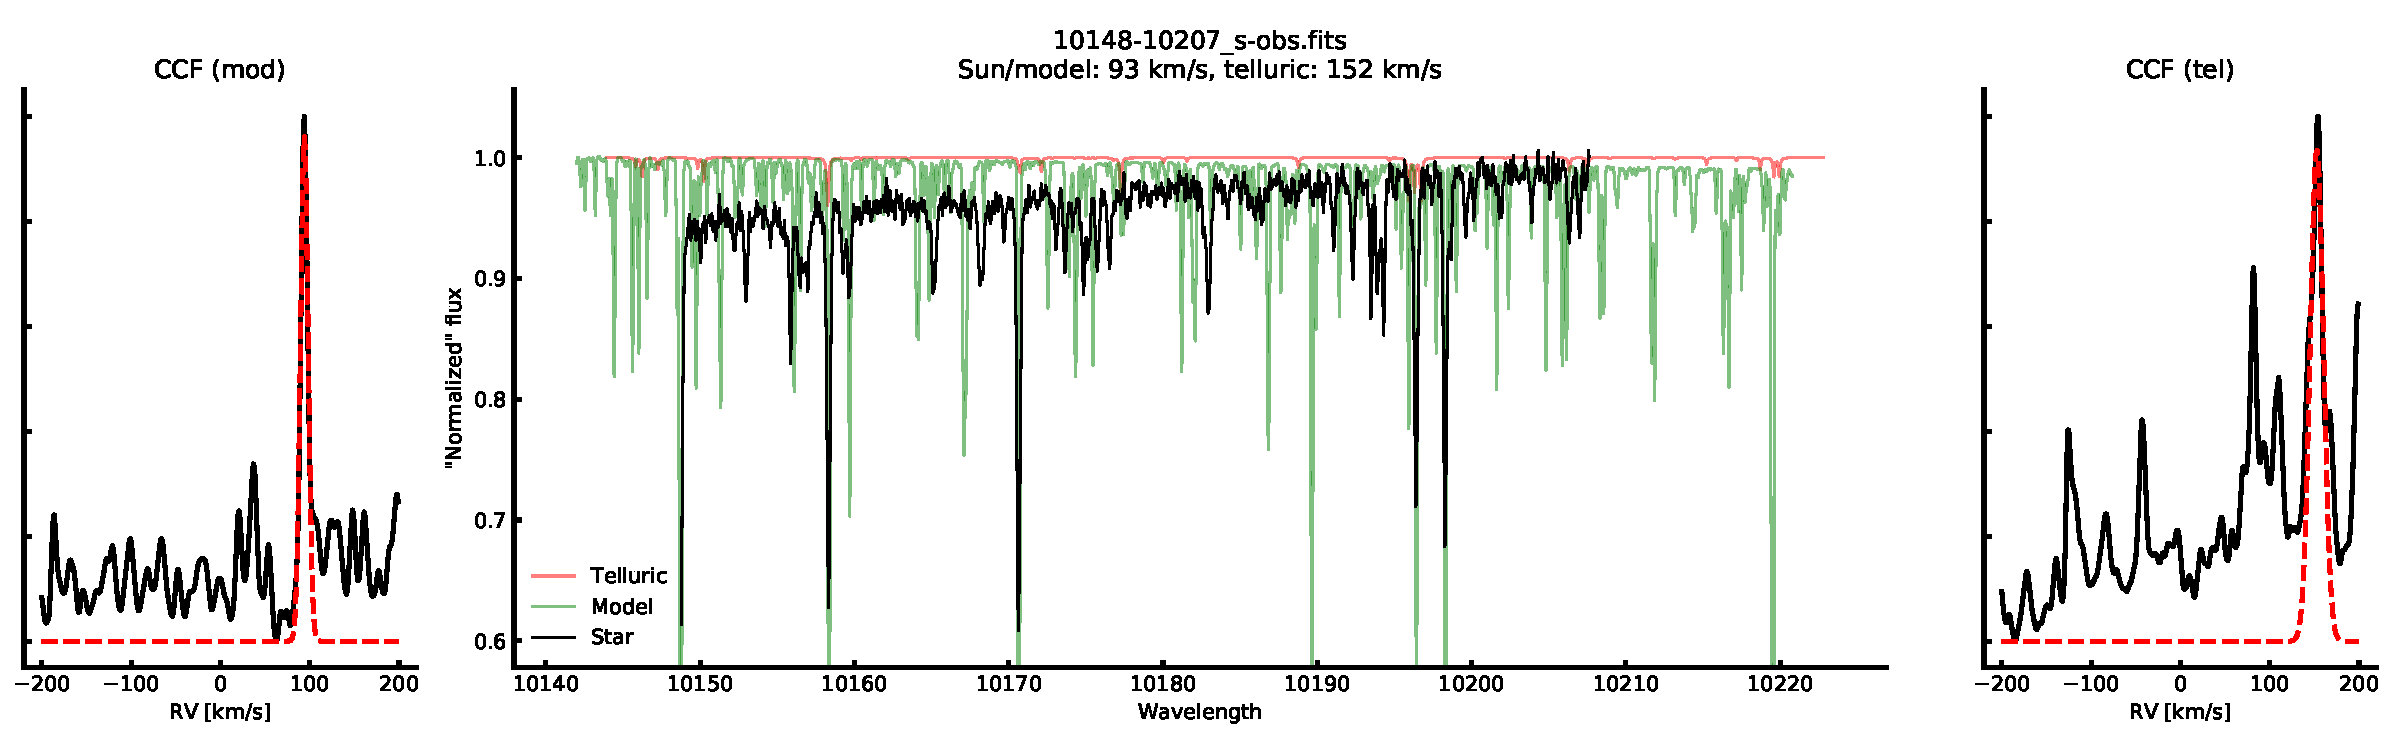
\includegraphics[width=1.0\linewidth]{figures/plot_fits.pdf}
    \caption{Line identification in piece of Arcturus spectrum with PHOENIX model and telluric model
             for correcting RV.}
    \label{fig:plot_fits}
\end{figure}
Once the lines were identified, the EWs were measured with the \code{splot} routine in \emph{Image
Reduction and Analysis Facility} (\code{IRAF}). The reason not to choose \code{ARES} for this task
was to visually confirm the identification of the line given the relative poor wavelength
calibration from the automatic pipeline. 249 \ion{Fe}{I} lines and 5 \ion{Fe}{II} EWs were measured
compared to 344 \ion{Fe}{I} lines and 13 \ion{Fe}{II} lines for the Sun over the whole NIR spectral
region in the line list. Whenever there were more than one EW measurement of a line, due to overlap
in different spectra, the average was used for the final EW. The stellar atmospheric parameters were
derived using the standard procedure (see \sref{sec:parameters}). Lines below \SI{5}{m\angstrom}
were removed in order to remove the lines which are most affected by contamination from either
telluric or other line blends. Additionally, a cut in EP at \SI{5.5}{eV} was made since the
\ion{Fe}{I} and \ion{Fe}{II} lines usually used for stellar parameter determination in the optical
regime are also limited to similar values \citep[see e.g][]{Sousa2008a}.

When deriving the stellar atmospheric parameters, one outlier were removed at a time (after a
completed minimization) until no outliers were present. Since we could only measure 5 \ion{Fe}{II}
lines, the parameter were also derived with $\log g=\SI{4.01}{dex}$ fixed at the reference mean
value (see \tref{tab:HD20010}). The resulting atmospheric parameters and iron abundances are
presented in \tref{tab:HD20010_results}. The effective temperature, surface gravity, and metallicity
agree within the errors with the literature values. Similar parameters are obtained by fixing $\log
g$ to the average literature value or by leaving it free.

\begin{table*}[htb!]
    \caption{The derived parameters for HD20010 with and without fixed surface gravity.}
    \label{tab:HD20010_results}
    \centering
    \begin{tabular}{lllll}
      \hline\hline
                     & $T_\mathrm{eff}$ (K) &  $\log g$ (dex)  &   $\xi_\mathrm{micro}$ (km/s)  & [Fe/H] (dex)      \\
      \hline
        Literature   & $6131 \pm 255$       &  $4.01 \pm 0.60$ &    $1.90 \pm 1.08$              & $-0.23 \pm 0.14$ \\
      \hline
                     & $6116 \pm 224$       &  $4.21 \pm 0.58$ &    $2.45 \pm 0.45$              & $-0.14 \pm 0.14$ \\
                     & $6144 \pm 212$       &   4.01 (fixed)   &    $2.66 \pm 0.42$              & $-0.13 \pm 0.29$ \\
      \hline
    \end{tabular}
\end{table*}

The errors on the atmospheric parameters for HD 20010 are much higher than what is achievable with
other measurements in the literature, as presented above in \tref{tab:HD20010}. In order to explain
these errors, the abundances for all lines which have at least two measurements of the EW were
calculated from the highest and lowest measured EW. The differences in abundances are presented in
\fref{fig:HD20010abundance}. The very large differences (more than \SI{0.1}{dex}) translate to the
high errors in the parameters.

\begin{figure}[htpb!]
    \centering
    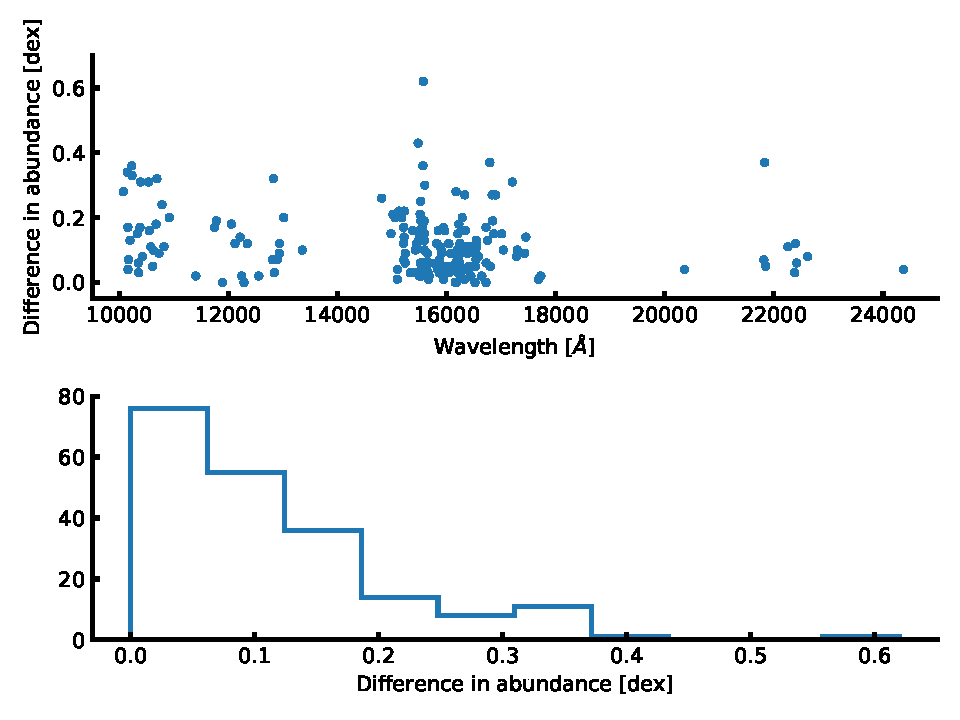
\includegraphics[width=0.8\linewidth]{figures/HD20010abundance_error.pdf}
    \caption{Difference in abundance for HD 20010 when multiple measurements of EW were obtained.
             The differences are between the lowest and highest measured EW in case of multiple
             measurements. This is shown against the wavelength (\emph{upper panel}) and in a
             histogram (\emph{lower panel}).}
    \label{fig:HD20010abundance}
\end{figure}

This test strongly suggest that errors in the EWs, likely due to the telluric contamination and
non-optimal reduction of the spectrum (poor default wavelength calibration), are responsible for the
relatively large error in the derived stellar parameters. After the first analysis of HD 20010, the
CRIRES-POP team published a fully reduced spectrum of 10 Leo \citep{Nicholls2017} with telluric
correction and an optimal wavelength solution. The results obtained from this star (see
\sref{sec:10Leo}) are very promising for the method used here, and it encourage a complete re-visit
of HD 20010 once the reduction is optimal.


\section{The NIR line list - toward cooler stars}
\label{sec:linelist_second}

As will be seen in \sref{sec:HD20010_first} the line list presented above was used to derive
atmospheric parameters of HD 20010. Even though the first test of the line list was successful, it
left room for improvements. The errors on the derived parameters were quite high for the spectral
type compared results obtainable with a similar analysis utilising the optical spectrum (see
\sref{sec:HD20010_first} for details on this). Additionally, the derived metallicity was
\SI{0.10}{dex} higher than the literature values used.

If all derived parameters except metallicity are reliable (when compared to e.g. a literature
value), then it suggest that the measured EW are either over- or underestimated. However, when using
a line list for the first time like here, it can also suggest problems with the line list itself,
most likely a bad calibration. This could have been wrong measurements of the EWs of the calibrator
star, Sun in this case. This combines to several cases:
\begin{itemize}
  \item Correct measurements of EWs of calibrator star:
  \begin{itemize}
    \item Systematic lower measurements of EWs of target star leads to underestimated $[\ion{M}/\ion{H}]$
    \item Systematic higher measurements of EWs of target star leads to overestimated $[\ion{M}/\ion{H}]$
    \item Correct measurements of EWs of target star leads to correct $[\ion{M}/\ion{H}]$
  \end{itemize}
  \item Systematic lower measurements of EWs of calibrator star:
  \begin{itemize}
    \item Systematic lower measurements of EWs of target star leads to underestimated $[\ion{M}/\ion{H}]$
    \item Systematic higher measurements of EWs of target star can lead to underestimated, correct or
          overestimated $[\ion{M}/\ion{H}]$ depending on the amount of systematic higher measurements
    \item Correct measurements of EWs of target star leads to underestimated $[\ion{M}/\ion{H}]$
  \end{itemize}
  \item Systematic higher measurements of EWs of calibrator star:
  \begin{itemize}
    \item Systematic lower measurements of EWs of target star can lead to overestimated, correct or
          underestimated $[\ion{M}/\ion{H}]$ depending on the amount of systematic lower measurements
    \item Systematic higher measurements of EWs of target star leads to overestimated $[\ion{M}/\ion{H}]$
    \item Correct measurements of EWs of target star leads to overestimated $[\ion{M}/\ion{H}]$
  \end{itemize}
\end{itemize}
It is important to note, that \emph{correct} has been used here, assuming a perfect setup, that
includes perfect model atmosphere, perfect radiative transfer code, etc. In reality the final
$[\ion{M}/\ion{H}]$ (and the other parameters) measured by different groups will occasionally differ
regarding the setup used \citep[see e.g.][]{Hinkel2016}.

As described in \sref{sec:linelist_first} the EW of the Sun (calibrator star) was measured with
\code{ARES}. A crucial option to set when using \code{ARES} is the \code{rejt} parameter as
mentioned in \sref{sec:measureEW}. This option is used to place the continuum and will thus directly
affect the measured EW. At the time of compiling the first version of the line list it seems the
\code{rejt} value used did not reflect the high S/N of the spectrum, thus placing the continuum too
low and thereby underestimate the EW. The \code{rejt} parameter used was 0.995 (S/N=200), while it
should have been closer to 0.999 (S/N=1000). This might have excluded some of the weakest lines,
since a cut in EW was made at \SI{5}{m\angstrom}.

In this second version of the line list, the goal is to:
\begin{enumerate}
  \item Make sure the EW measurements are as correct as possible by measuring them by hand
  \item Free of blended lines in cooler stars (K stars in this case)
\end{enumerate}
The second point is a similar exercise which was done in the optical by \citet{Tsantaki2013}, where
blended lines were removed from the larger line list by \citet{Sousa2008a}. This allowed to
determine the atmospheric parameters of stars colder than \SI{5000}{K}. However, the optical
spectrum still suffer for severely blended lines at low $T_\mathrm{eff}$, thus this method does not
work for M stars.

Both of the above steps were done at the same time, by measuring the EWs by hand using \code{IRAF}.
Whenever a line was difficult to reliably measure, i.e. a consistent measurement was not
possible/easy, it was discarded since it was blended. This can be seen in
\fref{fig:linelist_comparison} where the EW measurements from the first version is shown against
this version with the manual measurements. There are some measurements of EW higher than
\SI{150}{m\angstrom} which should have been removed. These lines have not been used during the
analysis, however they were kept since they might appear useful on a later stage.

\begin{figure}[htpb!]
    \centering
    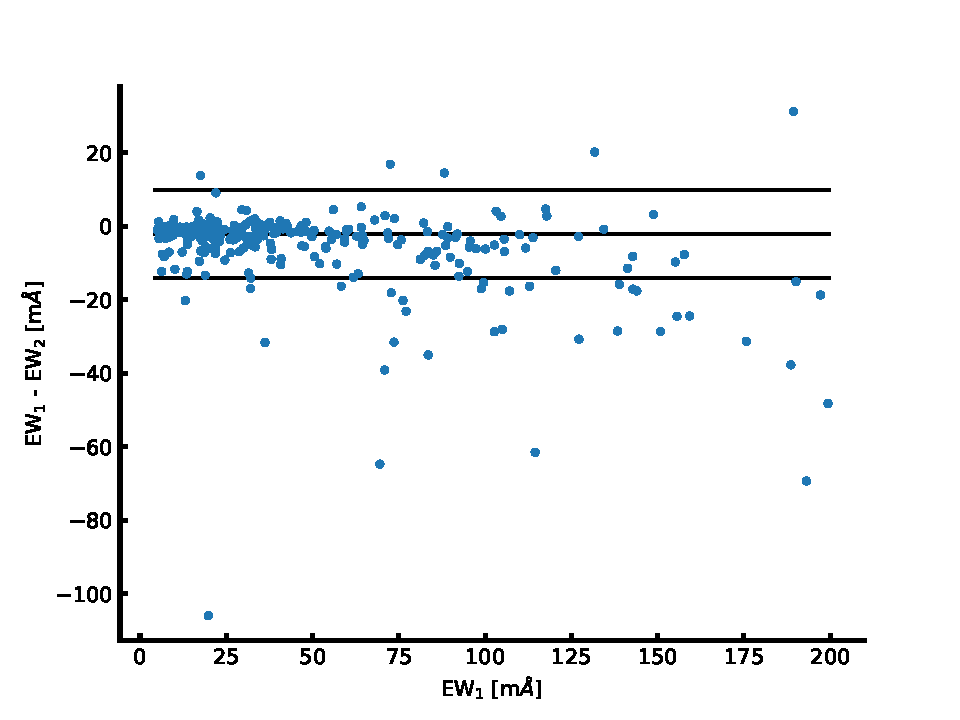
\includegraphics[width=1.0\linewidth]{figures/linelist_comparison.pdf}
    \caption{Comparison of the EW from the first version of the line list, EW$_1$, and the second
             version, EW$_2$. The EWs are generally higher in the second version, with an average
             difference between the two version of \SI{2.1+-11.1}{m\angstrom}. The three horizontal
             lines show the average value and the standard deviation.}
    \label{fig:linelist_comparison}
\end{figure}

With the increased access to high quality NIR spectra and the gained experience during the course
of the thesis, it was possible to improve the line list by a second visual inspection on the solar
spectrum.

After the new measurements of the EWs, the line list was re-calibrated according to the procedure
described above. The average change in $\log \mathit{gf}$ is $-0.062\pm0.157$, i.e. on average the
oscillator strengths are higher in the second version compared to the first version of the line
list.

With the second version there are only 5 \ion{Fe}{II} lines left which is a concern since these are
crucial for the derivation of the surface gravity.




\section{HD 20010 - revisited}
\label{sec:HD20010_second}

During the analysis of Arcturus (see \sref{sec:arcturus}) and 10 Leo (see \sref{sec:10Leo}) with the
refined line list presented in \sref{sec:linelist_second} it was a simple task to apply the updated
line list on HD 20010 a second time as a test whether it would perform similar, worse or better.
This is compared to results obtained from the literature and the previous results in
\sref{sec:HD20010_first}.

Therefore HD 20010 was revisited, and the atmospheric stellar parameters were derived. The measured
EWs from the results above in \sref{sec:HD20010_first} were kept, however the lines which did not
make the cut in the second version of the line list were removed. Moreover, the $\log \mathit{gf}$
values were updated since these were re-calibrated.

At this point \code{FASMA} was fully developed and was used to obtain the results which are shown in
\tref{tab:results} along with the results for Arcturus and 10 Leo (details on their parameters will
be found below). The agreement with the adopted average literature values are better for HD 20010
compared to the results from above in \sref{sec:HD20010_first} (especially $[\ion{Fe}/\ion{H}]$ and
$\log g$), and smaller errors with the updated results. This first test of the line list already
shows promising results. The literature values are slightly different here than compared to the
first analysis of this star. This is solely because other references were used, the PASTEL catalogue
\citep{Soubiran2016}. However, this does not change the improvement seen.


\begin{table}[htb!]
    \caption{Results for the three stars where first set of parameters are the literature values as
             presented in \tref{tab:stars}, second set of parameters are results with $\log g$ set
             to the same value during the minimization procedure as found in the literature (fixed),
             and last set of parameters are with all parameters free during the minimization
             procedure.}
    \label{tab:results}
    \centering
    \begin{tabular}{llll}
      \hline\hline
                                    & HD 20010          &  10 Leo           &  Arcturus        \\
      \hline
        Literature                  &                   &                   &                  \\
        $T_\mathrm{eff}$ (lit.)     & $6152 \pm  95  $  &  $4741 \pm  60  $ & $4300 \pm 110  $ \\
        $\log g$ (lit.)             & $3.96 \pm 0.19 $  &  $2.76 \pm 0.17 $ & $1.60 \pm 0.29 $ \\
        $[\ion{Fe}/\ion{H}]$ (lit.) & $-0.27 \pm 0.06$  &  $-0.03 \pm 0.02$ & $-0.54 \pm 0.11$ \\
        $\xi_\mathrm{micro}$ (lit.) & $1.17 \pm 0.24 $  &  $1.45 \pm 0.08 $ & $1.93 \pm 0.13 $ \\
      \hline
        $\log g$ fixed              &                   &                   &                  \\
        $T_\mathrm{eff}$            & $6161 \pm 164  $  &  $4761 \pm 118  $ & $4357 \pm  74  $ \\
        $\log g$                    & 3.96 (fixed)      &  2.76 (fixed)     & 1.60 (fixed)     \\
        $[\ion{Fe}/\ion{H}]$        & $-0.18 \pm 0.11$  &  $ 0.01 \pm 0.07$ & $-0.55 \pm 0.04$ \\
        $\xi_\mathrm{micro}$        & $1.72 \pm 0.44 $  &  $1.25 \pm 0.11 $ & $1.55 \pm 0.10 $ \\
      \hline
        All free                    &                   &                   &                  \\
        $T_\mathrm{eff}$            & $6162 \pm 184  $  &  $4805 \pm  98  $ & $4439 \pm  62  $ \\
        $\log g$                    & $4.08 \pm 0.77 $  &  $2.42 \pm 0.61 $ & $1.20 \pm 0.20 $ \\
        $[\ion{Fe}/\ion{H}]$        & $-0.18 \pm 0.11$  &  $-0.01 \pm 0.07$ & $-0.58 \pm 0.06$ \\
        $\xi_\mathrm{micro}$        & $1.59 \pm 0.49 $  &  $1.23 \pm 0.10 $ & $1.55 \pm 0.10 $ \\
        \hline\hline
    \end{tabular}
\end{table}




\section{Arcturus}
\label{sec:arcturus}

Arcturus is one of the brightest stars on the Northern hemisphere with a V magnitude of -0.05
\citep{Ducati2002}, and is well studied \citep[see e.g.][to mention just a
few]{Griffin1967,McWilliam1990,Ramirez2013}, and a benchmark star in current spectroscopic surveys
such as Gaia-ESO \citep{Jofre2014,Smiljanic2014}. Hence it is a prime target for testing with the
numerous measurements of the atmospheric parameters.

The atlas of Arcturus, acquired at Kitt Peak National Observatory using the FTS spectrograph at the
Mayall telescope by \citet{Hinkle1995a}, covers the spectral range of interest (YJHK bands). Strong
telluric features were identified with a spectrum from the TAPAS web page \citep{Bertaux2014} which
was useful during the line identification. The atlas also comes with a telluric standard and the
ratio of the two spectra in order to correct for the tellurics. The telluric spectrum from TAPAS was
only used for telluric line identification. Both the telluric corrected and non-corrected spectra
was used during the analysis, however the focus was on the non-corrected spectrum since it is simple
to identify the telluric lines in this spectrum.

The atlas consists of both a summer observation set and a winter observation set. The two data sets
have been obtained in order to minimise the effect of tellurics at different spectral regions. A
comparison between the two sets of measured EWs, both the manual measurements using \code{IRAF} and
the automatic measurements using \code{ARES}, are shown in \fref{fig:EWcomp}. The automatic EW
measurements for the summer set and winter set show excellent agreement with a dispersion of
\SI{7}{m\angstrom} and a systematic difference of \SI{0.1}{m\angstrom}, i.e. ineligible. This means
that the two data sets are very similar, thus it was decided to only manually measure the EWs for
one set (summer). Since this is a test of the line list (rather than a study of Arcturus) and the
fact that the EWs are very similar, the parameters are only derived from the summer set with the EWs
measured by \code{ARES}. Parameters were derived with and without $\log g$ set to a fixed value
(\SI{1.60}{dex}, the average literature value adopted). The derivation of the parameters followed
the same procedure as described above for HD 20010 using \code{FASMA}. Again outliers in abundance
were removed one at the time until there were no more outliers. The final results are presented in
\tref{tab:results} together with mean parameters from the literature.

\begin{figure}[htpb!]
    \centering
    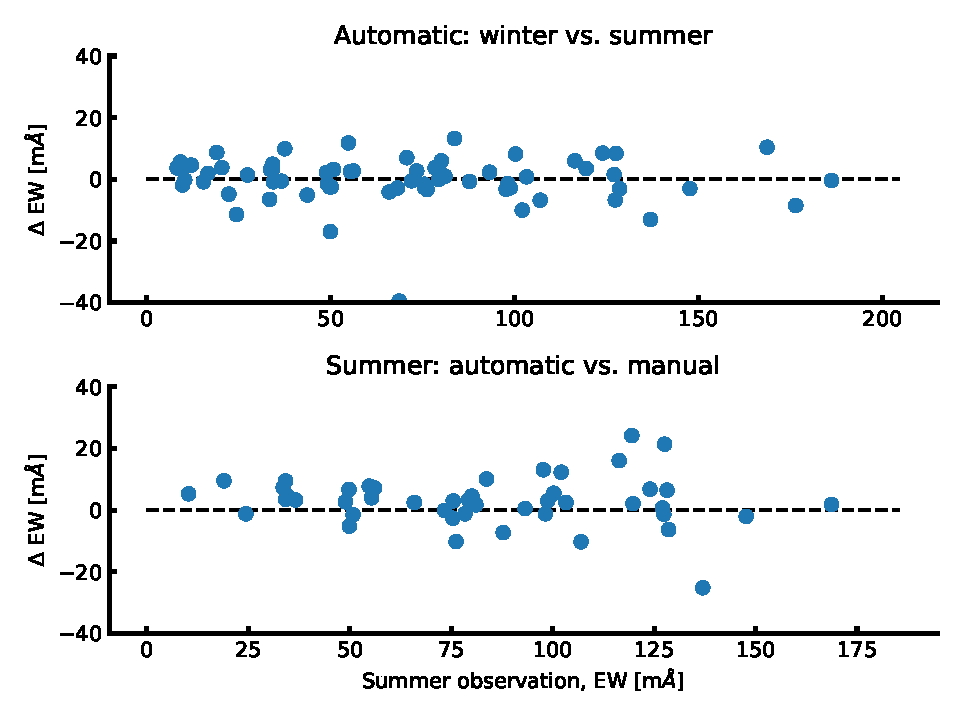
\includegraphics[width=1.0\linewidth]{figures/EWcomp.pdf}
    \caption{Top figure: Difference of the automatic EW measurements between the
             summer observations and winter observations from the Arcturus
             spectra. Bottom figure: Same as above, but with manual measurements
             from ARES (summer) and automatic measurements (summer).}
    \label{fig:EWcomp}
\end{figure}

There is overall good agreement between the derived parameters and the average values from the
literature adopted (see \tref{tab:results}). The only parameter being difficult to measure is the
surface gravity due to the low number of \ion{Fe}{II} lines in the NIR. This was already suspected
and mentioned in \sref{sec:linelist_second}. There are also some problems determining
$\xi_\mathrm{micro}$, however this is not a major concern, since it is not as important a parameter
as the other three. The derived metallicity is consistent with the literature here which is
promising since there were some problems with this parameter in \sref{sec:HD20010_first}.


\section{10 Leo}
\label{sec:10Leo}

The spectrum for 10 Leo was recently made available by the CRIRES-POP team \citep{Nicholls2017}. 10
Leo is very similar to Arcturus, which is also one reason this star was the first to be fully
reduced by the CRIRES-POP team. The spectrum is divided into several pieces according to the
atmospheric windows in the NIR: YJ (only together), H, K, L, and M. Here the first three were used
since this is the range of the line list. Some small gaps are present in the spectrum due to
tellurics that could not be properly removed, low S/N, bad pixels, etc. Rather than giving an
uncertain interpolation, \citet{Nicholls2017} decided to leave small gaps in the data. This had very
little effect on this line by line analysis, however, due to those gaps, one \ion{Fe}{II} line were
not measured which are crucial to determine the surface gravity.

The approach for determining the atmospheric stellar parameters for 10 Leo is identical to Arcturus.
\code{ARES} was used on each band (YJ, H, and K-band) separately. For the small gaps in the
spectrum, the flux was simply set to 1, since the spectrum has already been normalised. This also
prevented \code{ARES} to identify and measure any lines in these regions. The EWs from the three
regions were combined to one final line list used for the determination of the parameters. The final
results can be seen in \tref{tab:results}.

Generally the derived parameters are in excellent agreement with the literature values listed here.
A \SI{64}{K} difference is seen for $T_\mathrm{eff}$ with $\log g$ set as a free parameter, well
within the errors. The only parameter that show a discrepancy compared to the literature value is
$\xi_\mathrm{micro}$ with a difference of \SI{0.22}{km/s}, which is at the limit of the errors
reported. We note that this parameter is not reported in the PASTEL database\improvement{Then find
some reliable values instead}, and this was a derived parameter from an empirical relation. $\log g$
was derived with large errors which is a result from the few \ion{Fe}{II} (three lines) measured.
However, the $\log g$ is not far from the literature value, only \SI{0.34}{dex} lower, which is well
within the large errors reported. However, it also shows it is safer to obtain $\log g$ from other
more reliable methods, such as asteroseismology when possible.


\section{Synthetic cool stars}
\label{sec:synthetic_spectra}

Mainly due to lack of available high quality spectra in the NIR, it is a good test to use a
simulation. By deriving parameters from synthetic spectra, it is possible to carefully control the
work flow, in the sense that the target parameters are known. In this section the synthetic
library\footnote{\url{http://phoenix.astro.physik.uni-goettingen.de/}} by \citet{Husser2013} will be
used. These are synthetic spectra created from spherical symmetric PHOENIX atmosphere models under
local thermodynamic equilibrium. The model atmospheres does not include dust settling since all
models are hotter than \SI{2300}{K}. The details for the atmosphere models can be seen in
\citet{Husser2013}.

For this test only the $T_\mathrm{eff}$ will vary, ranging from \SIrange{3500}{6000}{K} with
most densely sampled at lower temperatures (see \fref{fig:phoenix_free}). Here $\log
g=\SI{4.5}{dex}$ and $[\ion{M}/\ion{H}]=\SI{0.00}{dex}$, i.e. synthesised dwarf stars with solar
metallicity. Before analysing the data, the spectra was broadened to have a spectral resolution of
\num{100000}, comparable with current and future high resolution NIR spectrographs.

In this test \code{ARES} was used to measure the EWs of as many lines from the line list (second
version) as possible for each of the 12 synthetic spectra. These line list were used to derive
parameters with two different model atmospheres, ATLAS9 \citep{Kurucz1993} and MARCS
\citep{Gustafson2008}, with \code{FASMA}. This was done twice, with all parameters derived from
\code{FASMA} (\fref{fig:phoenix_free}), and again with $\log g$ fixed at \SI{4.5}{dex} and
$\xi_\mathrm{micro}$ fixed which means it is changed in each iteration (see \sref{sec:parameters}
for details) according to an empirical relation. The latter case with fixed parameters is shown in
\fref{fig:phoenix_fix}.

\begin{figure}[htpb!]
    \centering
    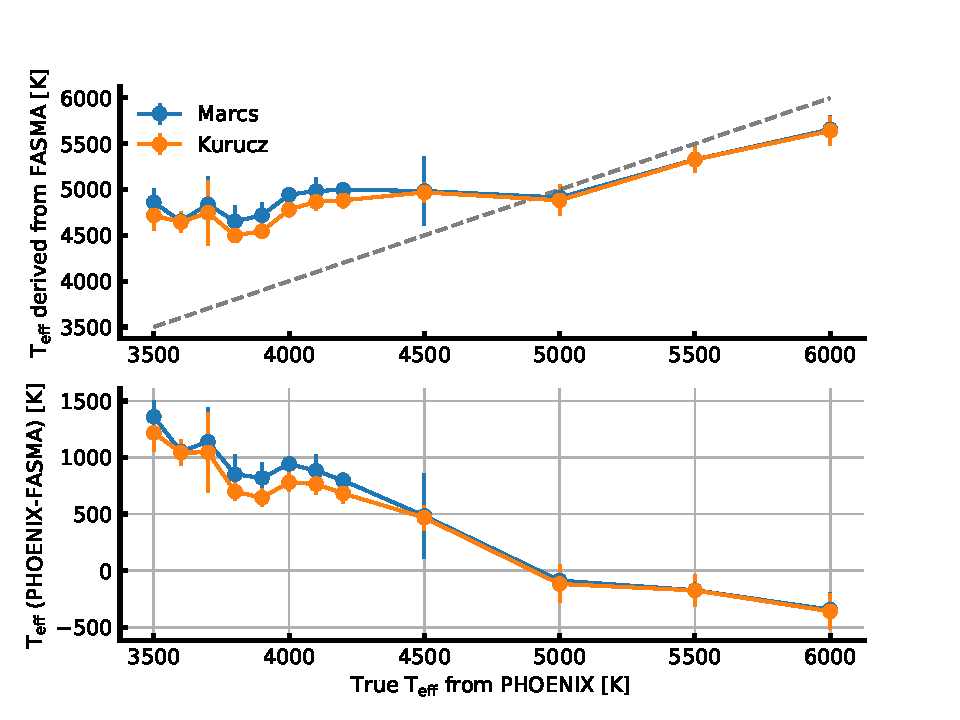
\includegraphics[width=1.0\linewidth]{figures/simulated_teff_free.pdf}
    \caption{Derived parameters of 12 synthetic PHOENIX spectra with varying $T_\mathrm{eff}$.}
    \label{fig:phoenix_free}
\end{figure}

For the results with $\log g$ and $\xi_\mathrm{micro}$ fixed at the correct parameters during the
derivation, the first thing noticed is the good agreement between the two model atmospheres. Second,
the derived $T_\mathrm{eff}$ are underestimated for $T_\mathrm{eff}>\SI{4000}{K}$ while for the two
lowest $T_\mathrm{eff}$ it is the opposite case. It is important to know that the grid of ATLAS9
models only go down to \SI{3750}{K}, however these synthetic spectra were included for completeness.
For $T_\mathrm{eff}>\SI{4000}{K}$ it is systematically lower by the same amount, roughly
\SI{100}{K}. As have been shown in the previous sections in this chapter, the methodology is
reliable for $T_\mathrm{eff}$ ranging from \SIrange{4300}{6200}{K} (see \tref{tab:results}). With
the consistent offset in $T_\mathrm{eff}$, it is a clear indication that the methodology is reliable
down to these temperatures.

In the case of $\log g$ and $\xi_\mathrm{micro}$ fixed the derived mean metallicity for the 12
synthetic spectra are $[\ion{Fe}/\ion{H}]=\SI{-0.12(17)}{dex}$ and
$[\ion{Fe}/\ion{H}]=\SI{-0.19(12)}{dex}$ for the ATLAS9 and MARCS model atmospheres, respectively.
The offset is likely to be found in the discrepancy between the model atmosphere and real data
(Arcturus in this case) as shown in \fref{fig:arcturus_phoenix}. Here a PHOENIX synthetic spectrum
with $T_\mathrm{eff}=\SI{4300}{K}$, $\log g=\SI{1.50}{dex}$, and
$[\ion{Fe}/\ion{H}]=\SI{-0.50}{dex}$ is plotted with a piece of the Arcturus atlas from
\sref{sec:arcturus}. The synthetic spectrum has similar parameters as Arcturus, thus they should
have similar spectral features. However, in the plot the spectral lines are deeper for the PHOENIX
model and there seem to be more absorption lines in this synthetic spectrum compared to the observed
spectrum. This have a direct effect on the measured EWs as they will be blended and deeper than
expected.


\begin{figure}[htpb!]
    \centering
    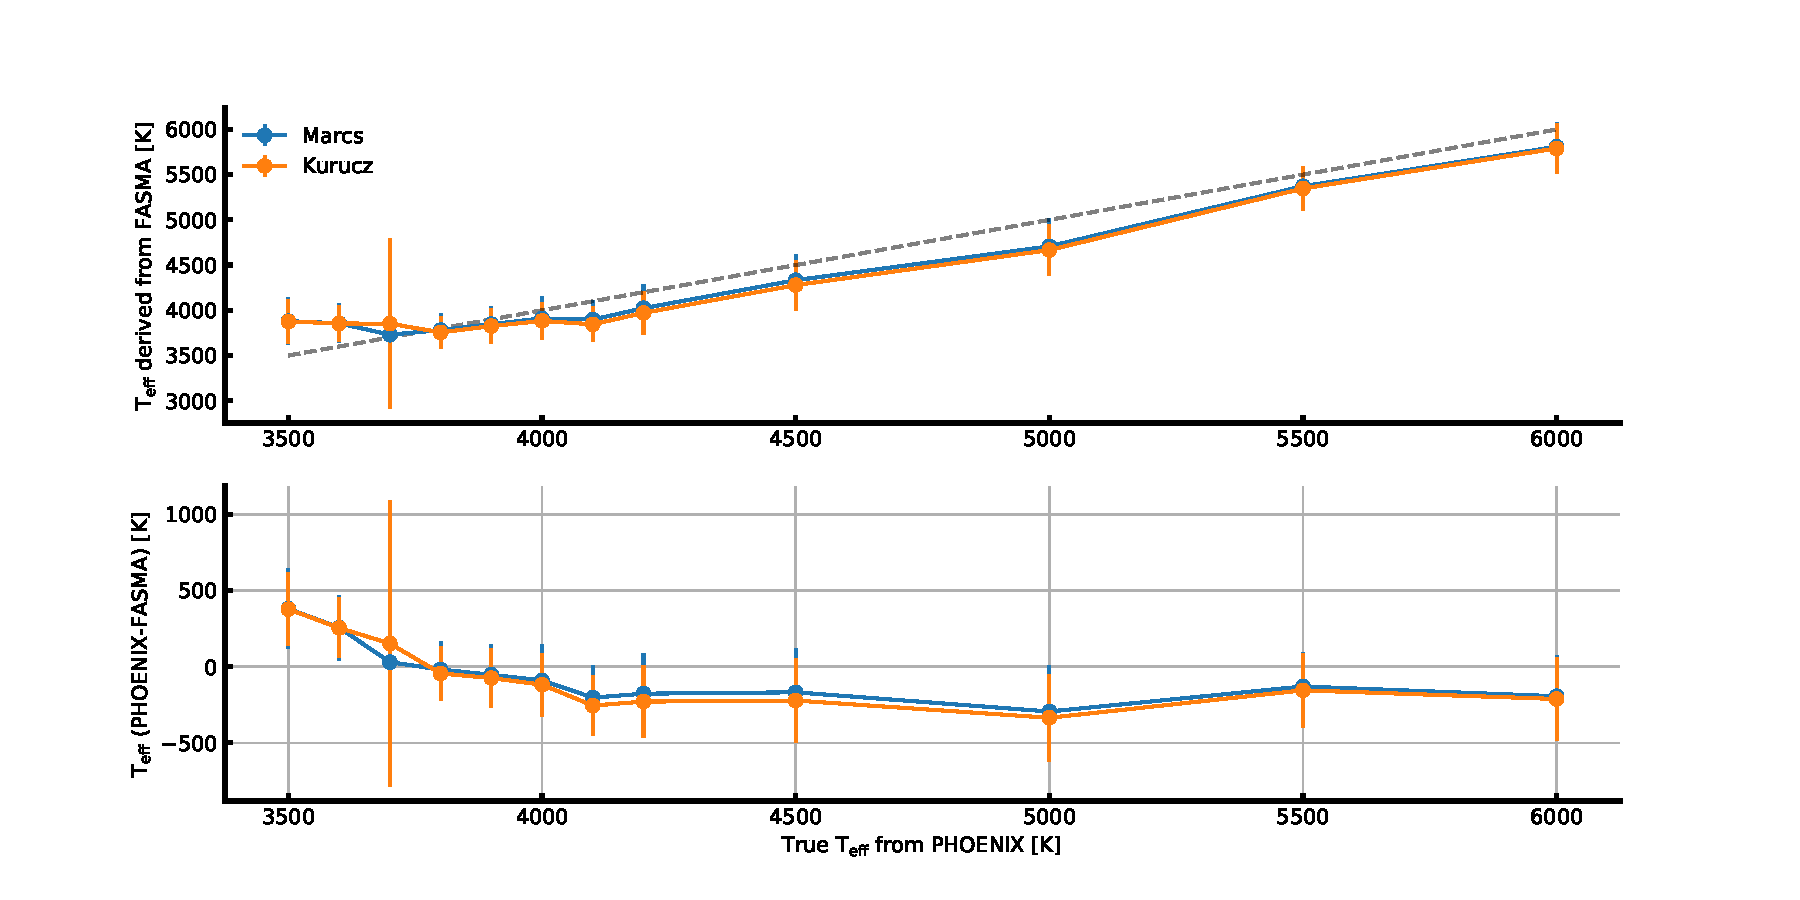
\includegraphics[width=1.0\linewidth]{figures/simulated_teff_fix.pdf}
    \caption{Derived parameters of 12 synthetic PHOENIX spectra with varying $T_\mathrm{eff}$. Here
             $\log g$ is fixed at \SI{4.5}{dex} and $\xi_\mathrm{micro}$ fixed according to an
             empirical relation, thus only deriving $T_\mathrm{eff}$ and $[\ion{Fe}/\ion{H}]$.}
    \label{fig:phoenix_fix}
\end{figure}

A comparison with EWs from the iron line list from the observed Arcturus spectrum and the
synthetic spectrum which resembles Arcturus closest is shown in \fref{fig:commonEWs}. The EWs are
clearly getting more disperse with increasing EW.

\begin{figure}[htpb!]
    \centering
    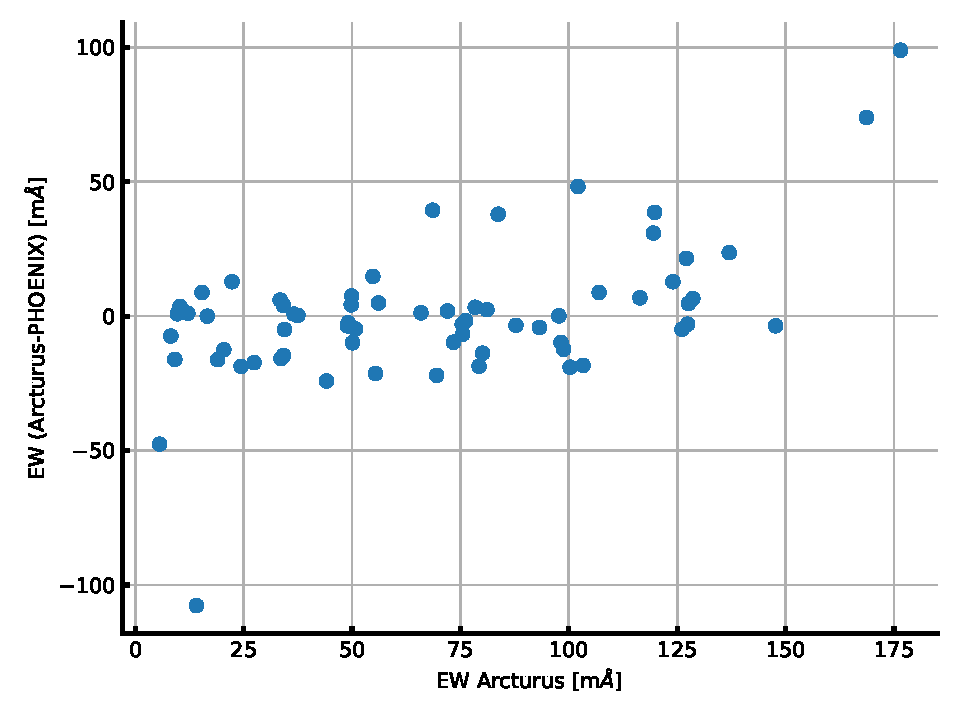
\includegraphics[width=0.8\linewidth]{figures/commonEWS.pdf}
    \caption{Common EWs between Arcturus and the synthetic spectrum with closest parameters (see
             text for details). The EWs are getting more disperse with increasing EW which is
             expected when seeing the direct comparison of the spectrum in
             \fref{fig:arcturus_phoenix}.}
    \label{fig:commonEWs}
\end{figure}

When all the parameters are derived it is a very different story for $T_\mathrm{eff}$. In this case
the $T_\mathrm{eff}$ are overestimated for the synthetic spectra colder than \SI{5000}{K}. Above
this limit the $T_\mathrm{eff}$ are slightly underestimated with a hint of the results getting worse
further from this limit. The reason for this can partly be found in the measured \ion{Fe}{II} lines.
As mentioned before, these are used to determine $\log g$. There have been measured between 1 and 3
\ion{Fe}{II} lines, generally fewer the lower $T_\mathrm{eff}$ is, out of 5 possible measurements.
The mean derived values for the surface gravity are $\log g=(1.11\pm1.63)\,\si{dex}$ and $\log
g=(1.38\pm1.45)\,\si{dex}$ for ATLAS9 and MARCS model atmospheres, respectively. Similarly for the
metallicity the following mean values are $[\ion{Fe}/\ion{H}]=\SI{-0.73(37)}{dex}$ and
$[\ion{Fe}/\ion{H}]=\SI{-0.73(38)}{dex}$ for ATLAS9 and MARCS model atmospheres, respectively.
The measured iron abundance for the 12 synthetic spectra can be seen in \fref{fig:feh_simulation}.
The figure only includes runs which reached convergence with \code{FASMA}.

\begin{figure}[htpb!]
    \centering
    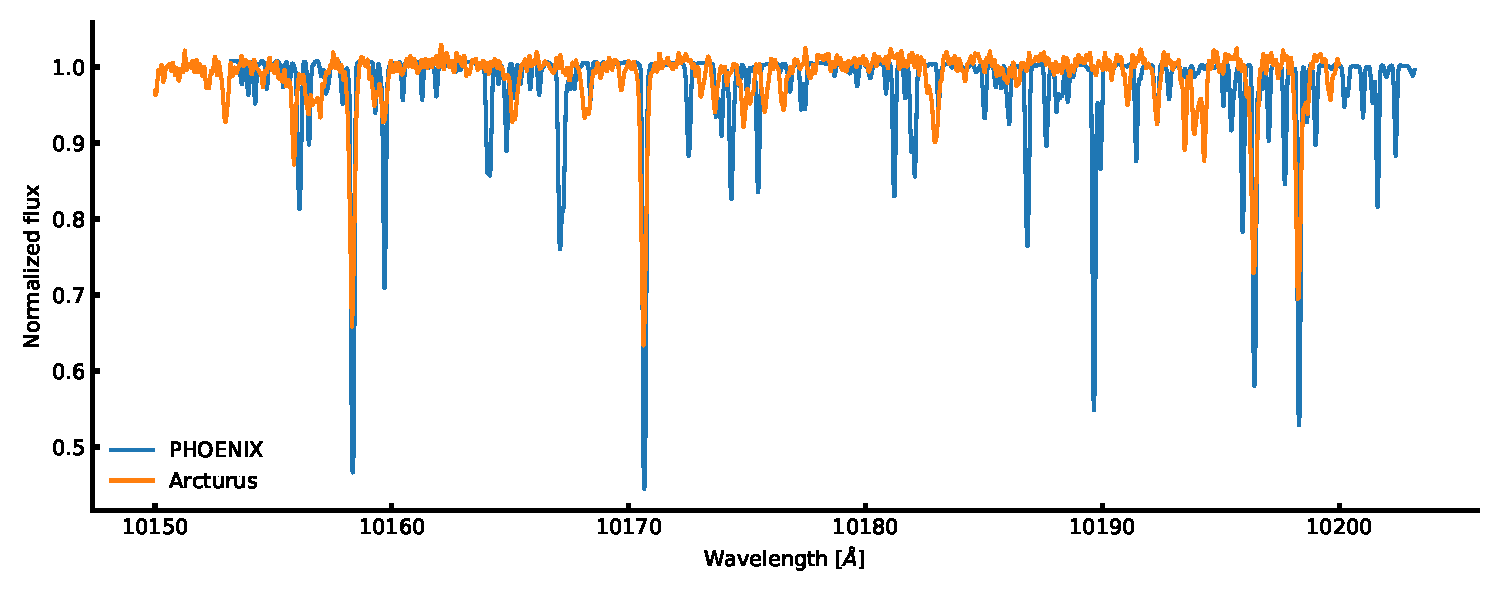
\includegraphics[width=1.0\linewidth]{figures/arcturus_phoenix.pdf}
    \caption{Comparison between the Arcturus atlas and a PHOENIX synthetic spectrum with similar
             parameters to Arcturus (see text for details).}
    \label{fig:arcturus_phoenix}
\end{figure}

\begin{figure}[htpb!]
    \centering
    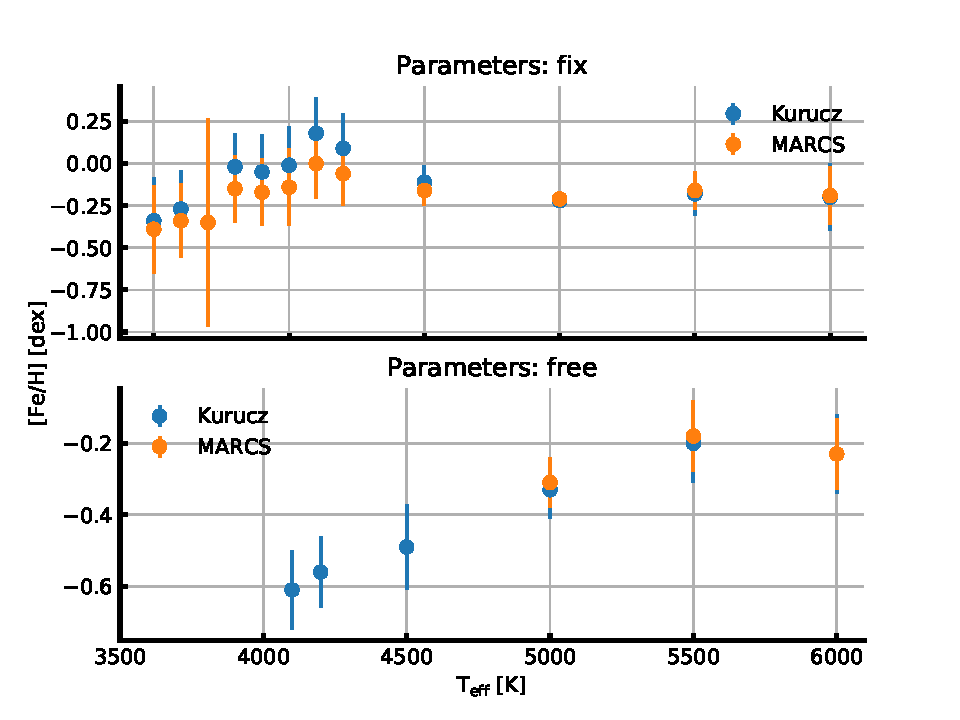
\includegraphics[width=1.0\linewidth]{figures/FeH_simulated.pdf}
    \caption{Derived $[\ion{Fe}/\ion{H}]$ with respect to the true $T_\mathrm{eff}$ for runs that
             reached convergence.
             \emph{Top panel}: $\log g$ fixed at \SI{4.5}{dex} and $\xi_\mathrm{micro}$ to the
             empirical relation (see text for details).
             \emph{Lower panel}: All parameters free.}
    \label{fig:feh_simulation}
\end{figure}
